% section 5: Results

\section{Results}

\subsection{Summary of DC2 runs}

In the course of executing DC2, we ran the pipelines over our input data
numerous times.  These runs uncovered a variety of bugs, performance
problems, and data quality issues which led to additional improvements
to the code.  Eventually, the maturity of the system was sufficient to
produce runs that would meet our objectives, so we have focused our
analysis of the results on three particular runs that featured
identical versions of the software: \code{rlp0127}, \code{rlp0128}, and 
\code{rlp0130}.  In these runs, the Image Processing and Detection
(IPD) pipeline featured 1 master pipeline process and 36 slice process
running across six nodes of the cluster.  The Moving Objects
Prediction System (MOPS) pipeline ran on node 9 with 3 slice
processes.  The Association pipeline ran on node 10 (where the
database was located) entirely in one process, the master process.
Each of these runs operated on a different set of 36 amplifier-sized
images from the same set of mosaic CFHT-LS D4 exposures (amplifier
numbers 73--108, 37--72, and 181--214, respectively).  From a total of
288 possible amplifier images per exposure, the amplifier sets were
chosen to sample different areas of the focal plan; \Fig{f6-1}
illustrates the location of these amplifier sets.  The number of 
visits completed in each run were 53, 62, and 62, respectively, for a
total of 177 visits.   A summary of the three runs, including the
number of images successfully processed, appears in \Table{t6-1}.  

\begin{figure}[htbp]
\begin{center}
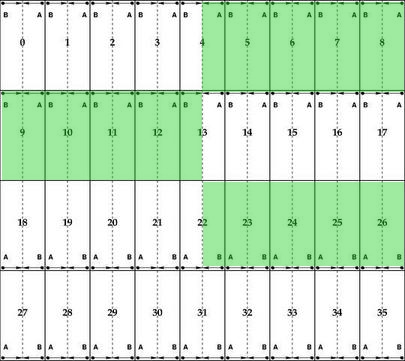
\includegraphics[height=60mm] {figures/MegaCamMap}
\caption{Map of the CFHT MegaCam focalplane.  The area covered by DC2
  runs rlp0127, rlp0128, and rlp0130 are shown in green\label{f6-1}}
\label{FigMegaCamMap}
\end{center}
\end{figure}

\begin{table}[htbp]
\begin{center}
\caption{Summary of DC2 Reference Runs\label{t6-1}}
\vspace{\baselineskip}
\begin{tabular}{ | r | r | r | c | r | r | r |}
\hline
runId & nVisits & nAmps & Amp IDs & inputImages & outputImages & outputFrac \\ \hline
rlp0127 & 53 &  36 &  73-108 & 1908 & 1875 & 0.983 \\ \hline
rlp0128 & 62 &  36 &  37-72  & 2232 & 2228 & 0.998  \\ \hline
rlp0130 & 62 &  36 & 181-214 & 2232 & 2213 & 0.991 \\ \hline
Total   & --- & 108 &   ---    & 6372 & 6316 & 0.991 \\ \hline
\hline
\end{tabular}
\end{center}
\end{table}

We note that the DC2 pipeline will run without modification on much
larger clusters.  A cluster with 288 cores would allow the full CFHT
MegaCam mosaic to be processed in parallel.  We expect such hardware
to be available to us very soon, and we will supplement this report
with results from such runs when they are available.

\subsection{Science data quality}
\label{ScienceDataQuality}

We did not set explicit science data quality criteria for DC2.
Nonetheless, it is valuable to briefly consider the topic here, since it gives
us guidance in planning for DC3.  The main role of the nightly
processing pipelines in the overall LSST data flow is to generate
transient alerts.  These alerts will be based on the DIASources produced by
the IPD pipeline and associated with Objects by the Association
pipeline. Although the alert generation logic is still to be designed,
it is clear that it will rely in part on the lightcurves of candidate
Objects, since they give the history of the Object's behavior.  A key
science metric, therefore, is the quality of these lightcurves.

Taking the results from rlp0128 as representative of the three runs
that made up DC2, a total of 72569 DIASources were generated.  The
histogram of the number of DIASources per Visit is shown in \Fig{FigDIAHist},
and of the number of lightcurve points for an Object in \Fig{FigDIALCHist}.  Two
points are clear from these plots:

\begin{itemize}
\item{A few visits generate anomalously large numbers of DIASources; and}
\item{The vast majority of Objects have only a single lightcurve point.}
\end{itemize}

\begin{figure}[htbp]
\begin{center}
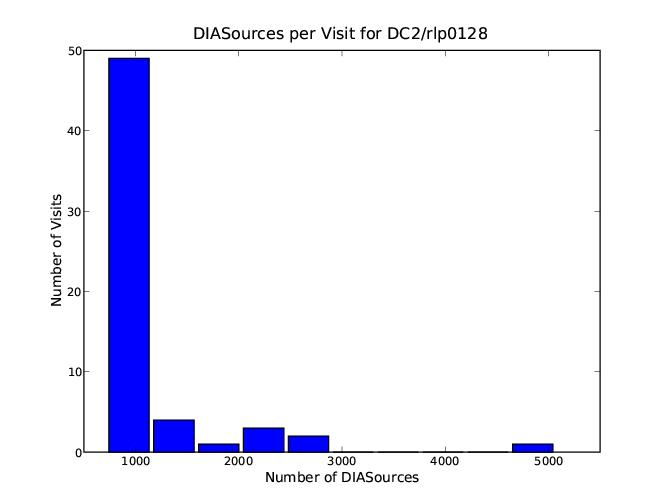
\includegraphics[height=60mm] {figures/VisitHisto_rlp0128}
\caption{Histogram of the number of DIASources per Visit for DC2 run \code{rlp0128}
\label{FigDIAHist}}

\vspace{0.1\textheight}

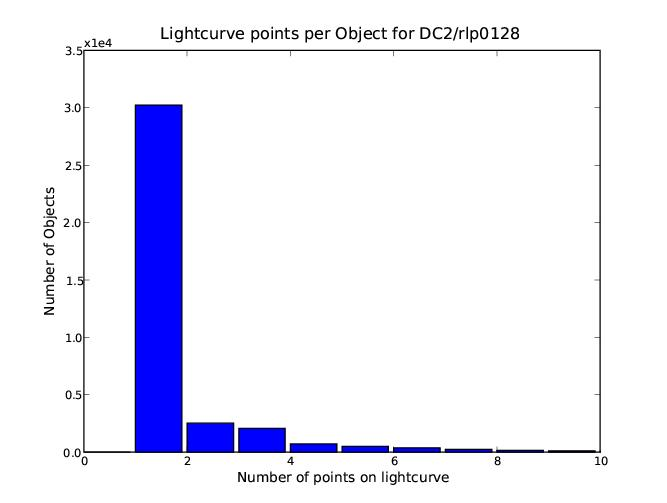
\includegraphics[height=60mm] {figures/LCHisto_rlp0128}
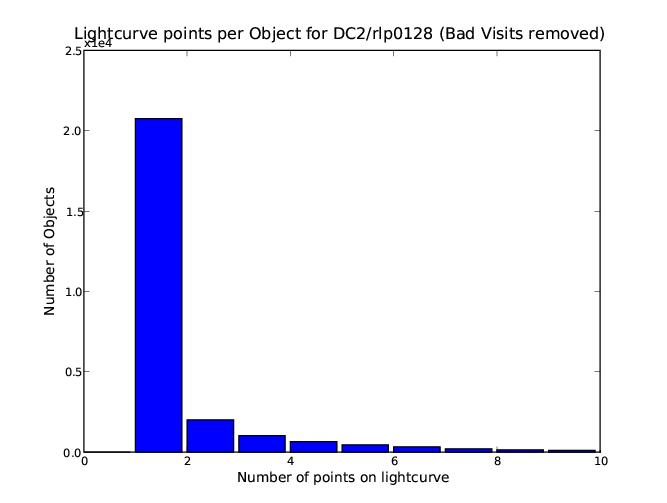
\includegraphics[height=60mm] {figures/LCHistoClean_rlp0128}
\caption{Histogram of the number of DIASources per Object for DC2 run
  \code{rlp0128}.  This is the number of points on the lightcurve for the
  Object. On the right, after eliminating Visits that produced more than 2000 DIASources.
  Note that the ordinate is in units of $10^4$.
\label{FigDIALCHist}}
\end{center}
\end{figure}
  
Inspection of the images shows that the anomalous Visits reflect a
variety of problems in the input images themselves, or in the
subtraction process.   These include template images that are severely
misregistered with their science image. A replot of the lightcurve
point histogram with anomalous Visits (defined as those producing \ensuremath$>2000$
 DIASources) is shown in \Fig{FigDIALCHist}.   There are substantial
reductions in the number of lightcurves with 1, 2, or 3 points, but
qualitatively the picture is unchanged.

Analysis of individual lightcurve quality is time consuming, since the
image region corresponding to each individual point must be assessed
(at the moment, by eye).   At present, only a small fraction of the
available lightcurves have been checked, drawn from representative
points on the  \Fig{FigDIALCHist} histograms, leading to the following
preliminary conclusions:

\begin{itemize}
\item Lightcurves with only a single point are overwhelmingly due to
  cosmic rays.  These will be effectively eliminated in DC3 by
  incorporating cosmic ray rejection into the detection stage of the
  IPD pipeline (cf. \Fig{FigCRbefore}), and further in LSST by the use of two Exposures per
  Visit.
\item The majority of the remaining lightcurves come from ``bipolar''
  subtractions, in which the subtracted image contains a closely
  spaced pair of peaks, one positive and the other negative.   These
  result from poor subtraction kernels.  A number of causes of these
  are understood, and discussed in \Sec{sApp-imsub}.
\item A small number of lightcurves resulting from variable stars are
  present in the data.   The individual DIASources are being correctly
  associated with their Object by the Association pipeline.  The
  fluxes being produced by the Detection stage of the IPD pipeline
  appear to be noisy, however.  Some causes of this are also discussed
  in \Sec{sApp-imsub}.
\end{itemize}

\subsection{Timing results}
\label{sRes-time}

Because the Logging framework attaches a timestamp to every logging
message, we can use it to instrument the pipeline harness and
calculate the time spent in various parts of the pipeline.  In
particular, we inserted logging calls to mark the beginning and end of
important sections of the pipeline processing, such as the start and
end of the process function for each stage.  This technique allowed us
to separate out the different contributions to the overall processing
time, including I/O, middleware overhead, and time spent running
scientific algorithms.  This section presents the results of this
analysis.  

Among the logging markers we included in the harness code was a mark
indicating the start of processing of each visit.  Thus the total cost
of processing each visit was determined by calculating the time
between each such mark.  The average of these times are shown in Table
\ref{t6-2}.  As we will see, the variation is not Gaussian (as they are
certainly dominated by systematic effects), so the calculated standard
deviation is just indicative of the spread in values.\placetable{t6-2}
The variation is better seen in the \Fig{f6-4}.  

\begin{deluxetable}{lrr}
\tablecaption{Average time to process one visit through each pipeline.\label{t6-2}}
\tablewidth{0pt}
\tablehead{
\colhead{Pipeline} & \colhead{avg. time (s)} & \colhead{$3\sigma$ (s)}
}
\startdata
Image Processing/Detection (IPD) &  207.2 & 108.2 \\
Moving Objects (MOPS)            &   52.9 &   4.1 \\
Association                      &  207.4 & 108.5 \\
\enddata
\\[-1.5\baselineskip]
\tablecomments{$N_{visits}=177$}
\end{deluxetable}

\begin{figure}[htbp]
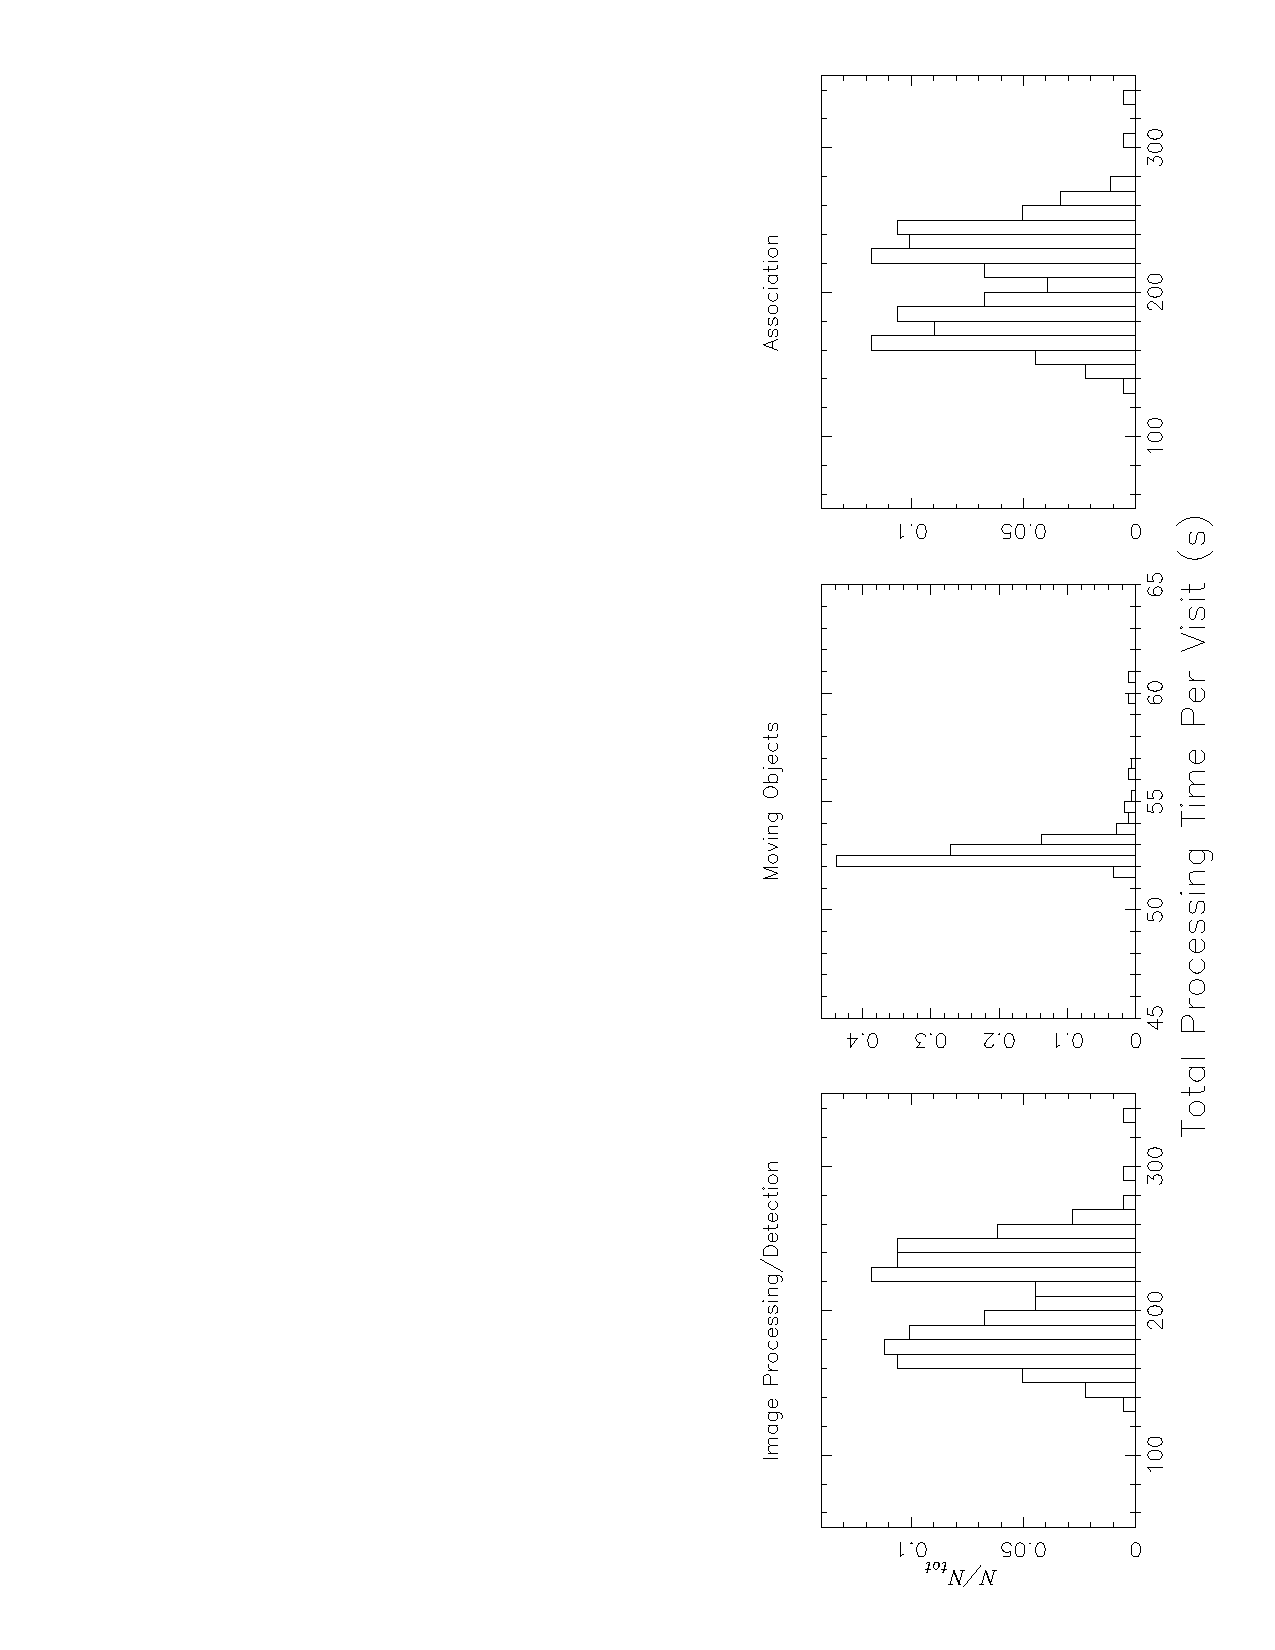
\includegraphics[width=0.8\textwidth,angle=-90,scale=0.375,viewport=364 29 583 757,clip]{figures/MasterLoopHist.pdf}
\caption{Histogram of the times to process each of visit.  The
  $y$-axis measures the fraction of the 177 visits in each time bin.\label{f6-4}} 
\end{figure}

One of the most notable features of the graphs is the correlation
between the IPD data and the Association data.  This reflects the fact
that the Association pipeline pauses at the beginning of each visit to
await an event sent from the IPD pipeline in its last stage signalling
the availability of new detections.  Consequently, the total time spent
processing a visit in the Association pipeline is dominated by this
wait time.  \Fig{f6-5} illustrates only the time spent in
Association application code.  The time spent by the pipeline
framework managing the pipeline, including the spent waiting for
events, has been excluded.  As we can see, this time is much less than
that shown in \Fig{f6-4}.  (As we will see later, the contribution of
the middleware overhead is even smaller.)  The mean time of this set
is 6.9~s.  

\begin{figure}[htbp]
\begin{center}
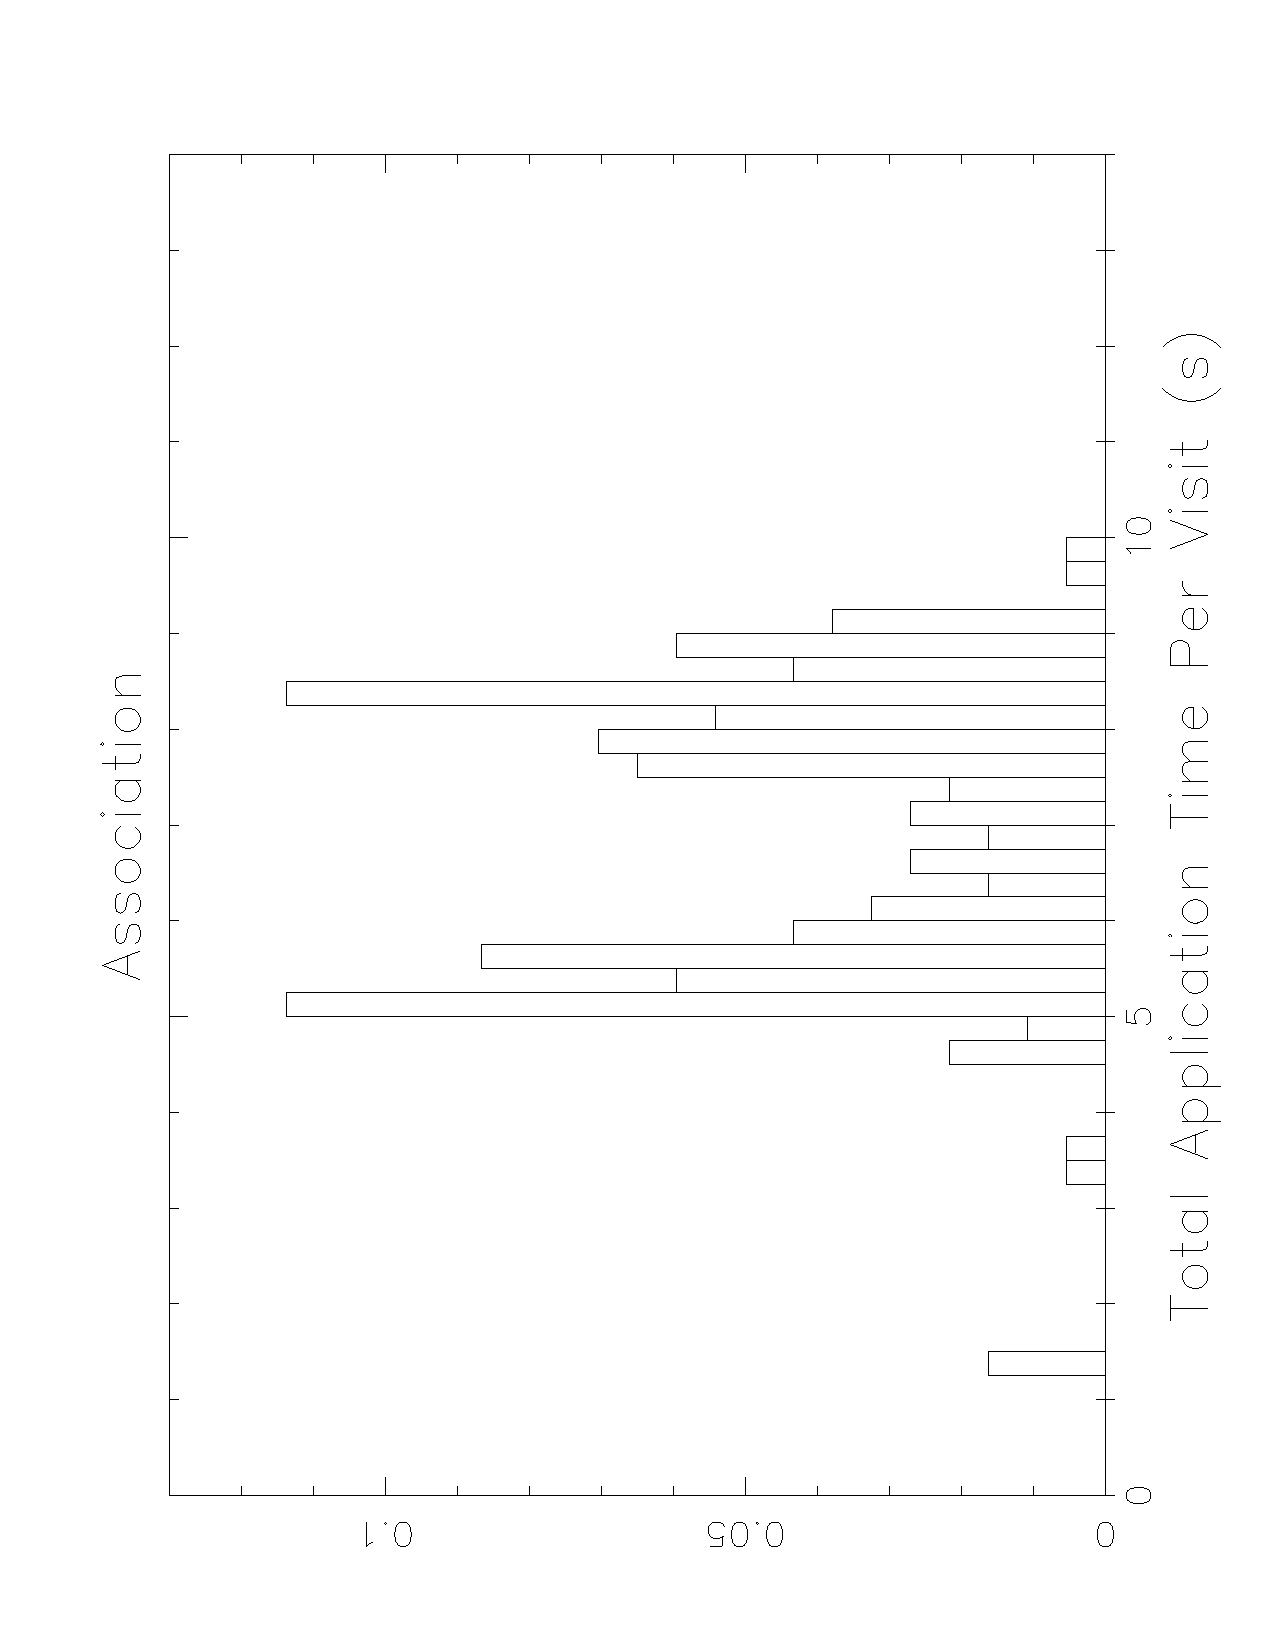
\includegraphics[width=0.8\textwidth,angle=-90,scale=0.45,viewport=47 49 587 719,clip]{figures/AppLoopHistAssoc.pdf}
\end{center}
\caption{Histogram of the times applying the association algorithm to
  each visit, excluding the time waiting for an event and the time
  spent managing the pipeline.  The $y$-axis measures the fraction of 
  the 177 visits in each time bin.\label{f6-5}} 
\end{figure}

\begin{table}[htbp]
\begin{center}
\caption{Average application processing time per stage (s)}
\label{t6-3}
\vspace{\baselineskip}
\begin{tabular}{crccrcr|crcr|crcr}
\tableline\tableline
&&& \multicolumn{4}{c|}{IPD} & 
    \multicolumn{4}{c|}{MOPS} & 
    \multicolumn{4}{c}{Association} \\
\multicolumn{3}{c}{Stage} 
&\multicolumn{3}{c}{average}&\multicolumn{1}{c|}{$3\sigma$} 
&\multicolumn{3}{c}{average}&\multicolumn{1}{c|}{$3\sigma$} 
&\multicolumn{3}{c}{average}&\multicolumn{1}{c}{$3\sigma$} \\
\tableline
& 1 && &   0.023 &&  0.082 & 
       &   0.010 &&  0.008 &
       &   0.460 &&  0.162   \\
& 2 && &   9.567 &&  2.598 &
       &  52.399 &&  2.886 &
       &   0.156 &&  0.210   \\
& 3 && &   0.027 &&  0.015 & 
       &   0.039 &&  0.144 &
       &   0.024 &&  0.040   \\
& 4 && &   0.039 &&  0.007 & 
       &   0.056 &&  0.022 &
       &   0.040 &&  0.024   \\
& 5 && &   7.023 &&  2.411 &&&&&
       &   0.018 &&  0.004   \\
& 6 && & 175.141 && 99.467 &&&&&
       &   0.018 &&  0.005  \\
& 7 && &   6.489 &&  2.016 &&&&&
       &   0.037 &&  0.023  \\
& 8 && &   7.521 && 35.196 &&&&&
       &   6.136 &&  4.741  \\
& 9 && &   0.133 &&  1.119 &&&&& &&& \\
&10 && &   0.061 &&  0.008 &&&&& &&& \\ 
\tableline
\end{tabular}
\end{center}
\end{table}

The obvious conclusion from the results shown thus far is that the
IPD pipeline is the source of the most costly processing.  We narrow
down the source of the bottlenecks in \Table{t6-3} in which we
plot the processing time as a function of pipeline stage for each
pipeline.  From this table, we can see:
\begin{itemize}
\item The costliest stage of the IPD pipeline is stage 6 that does
  the image subtraction.  
\item The next costliest IPD stage, on average, is stage 2 that
  reads the input images into memory; however, the time spent in stage
  7 which does source detection can vary quite a bit, sometimes
  dominating over stage 2.  This depends on the number of sources
  detected in the subtracted image. In the worst cases the subtraction
  was such that the detected sources comprised most of the pixels
  in the image.
\item Stage 2 of the MOPS pipeline is where the ``day-MOPS'' algorithm
  is applied (as the others handle I/O), so as expected this stage
  dominates the processing costs.  
\item The dominant stage of the association pipeline is Stage 8 which
  updates the source catalog.  
\item The association pipelines source matching stages, 3 and 6, are
  relatively fast, typically taking under 0.1 s.  
\end{itemize}

Because the image subtraction contributes such a large fraction of the
overall run time, we undertook a more detailed analysis of its time
usage.  This indicates that the convolution of the template image with
the spatially varying kernel is taking the bulk of the time.   A
simple convolution test case with a spatially invariant kernel
indicates that the current code is running at least a factor of 10
slower than is achieved by existing optimized convolution codes.  We are
working to understand the causes of this, which are certainly
connected to the compiler's treatment of pixel access in the vw
library.  We fully expect to attain full performance from relatively
minor modifications to the vw code, possibly combined with some
changes in the way we utilize it for convolution.

The time spent in stage 6 of the IPD pipeline is dominated by the 
\code{process()} step.  More precisely, because all of the slices
synchronize at the end of this step --- that is, the master process waits
until all of the slices have finished their processing before
proceeding on to the \code{post-process()} step --- the total time spent
in the stage is always longer than the processing time of the slowest
slice.  Looking at all the times spent in the \code{process()} step of
stage 6, we see a large variation.  \Fig{average-node-time} shows the
average time spent on this step as a function of node.  Clearly the
best performing nodes are 5--8 which are the newest machines in the
cluster.  The slices on the older node 1 ran over twice as slow on
average as those on the newer node, and the slices on node 4 ran about
50\% slower.  We might surmise that if we had a homogeneous cluster
consisting all of the newer blades we would see IPD running on average
about 70 s per visit.  We note that the variation of processing times
is still quite large for slices on the newer nodes, suggesting that
peculiarities in the data itself can still have a big effect on the
processing time.

To confirm our hypothesis regarding a homogeneous cluster, we did a
run in which the IPD pipeline only used nodes 5--8.  The average time
spent on image subtraction was 72.7~seconds (with a full range of 33.5
to 122.4~seconds) which is consistent with \Fig{average-node-time}.
The variation is still large, and at least one slice significantly
slows down the processing of the entire exposure.  This could be due
to variations in the data itself, or it could be an effect of running
multiple slices on the same multi-core node.  This latter possibility
could be tested by examining how the processing times change as a
function of the ratio of the number of slices deployed on a node
vs. the number of available cores.  

\begin{figure}[htbp]
\begin{center}
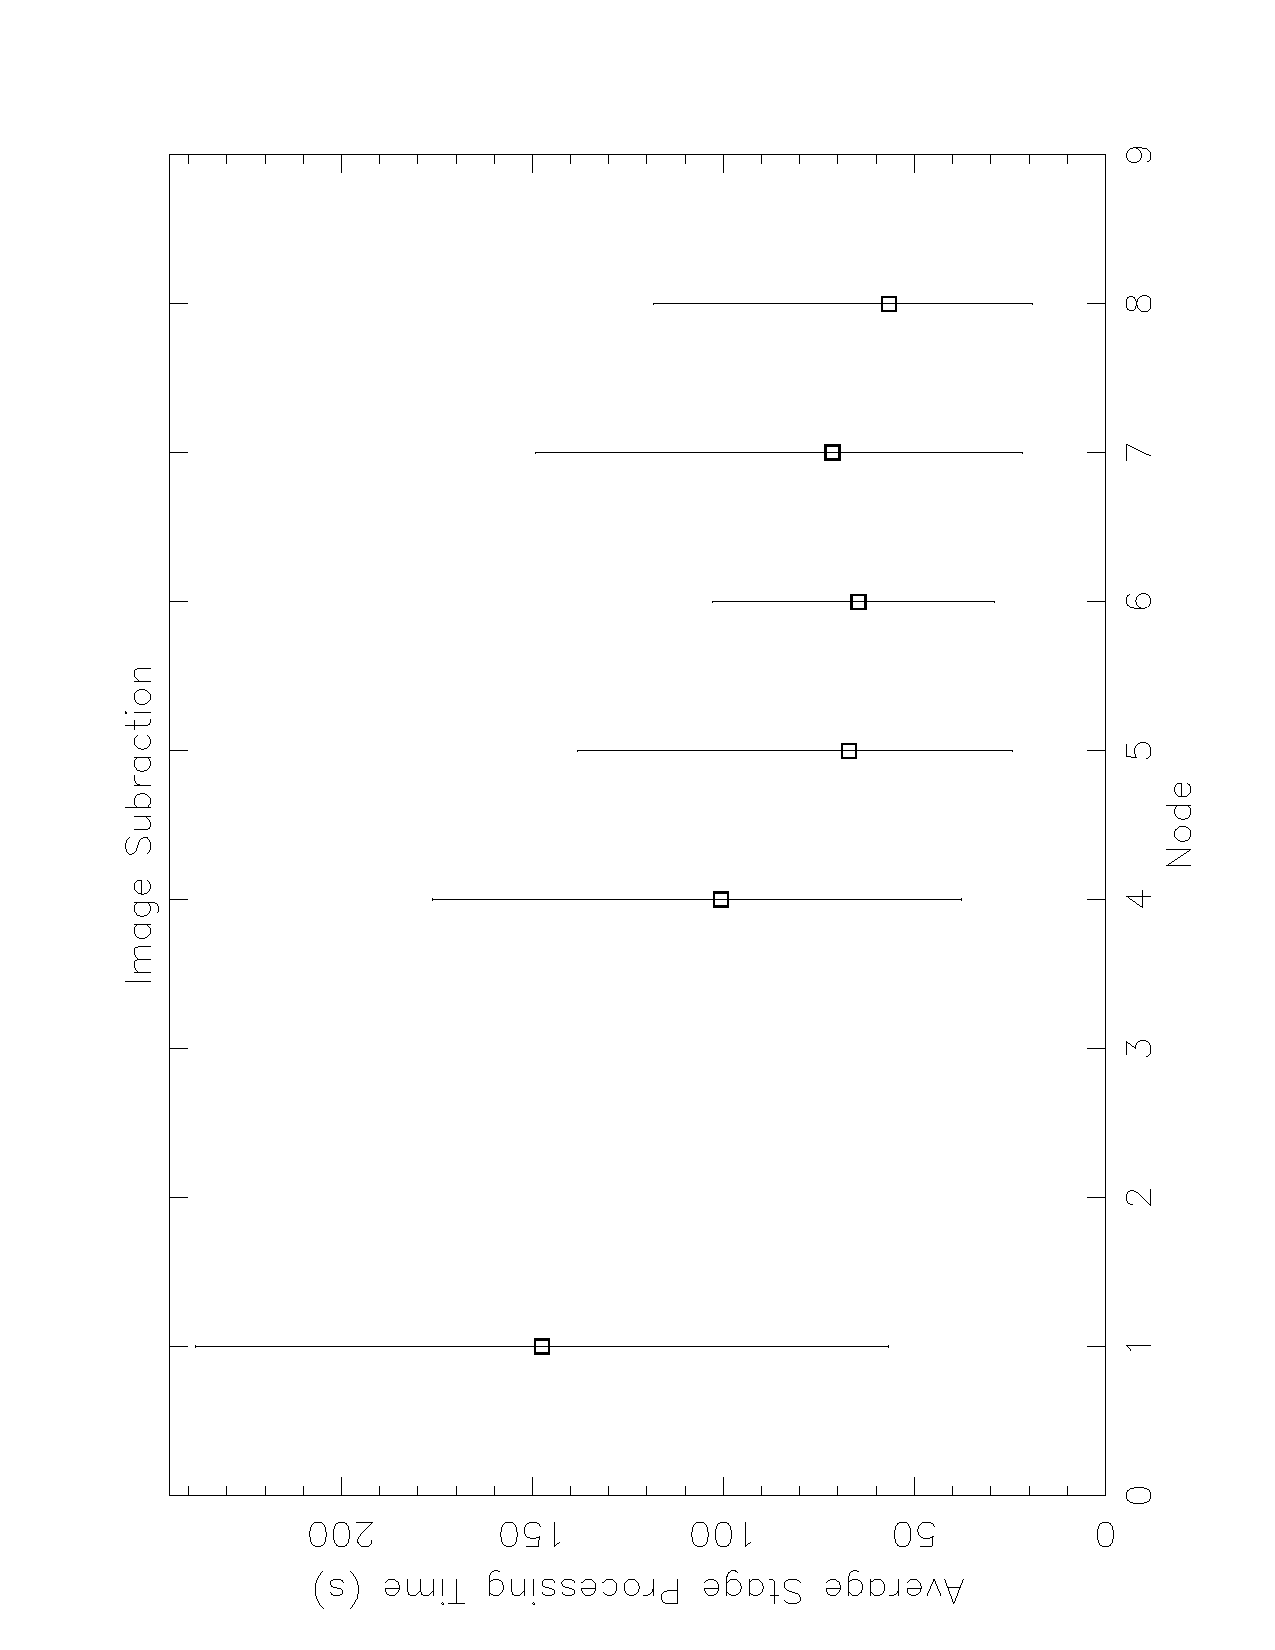
\includegraphics[width=0.8\textwidth,angle=-90,scale=0.45,viewport=59 19 572 722,clip]{figures/StageProcVsNode.pdf}
\caption{A plot of the average time (represented by the squares)
  spent within the \code{process()} step of the IPD pipline's stage 6
  as a function of node.  The bars passing through each square extend
  to the minimum and maximum times measured on that node.  Nodes 1--4
  are older, less powerful machines than nodes 5--8.
\label{average-node-time}} 

\vspace{0.5\baselineskip}

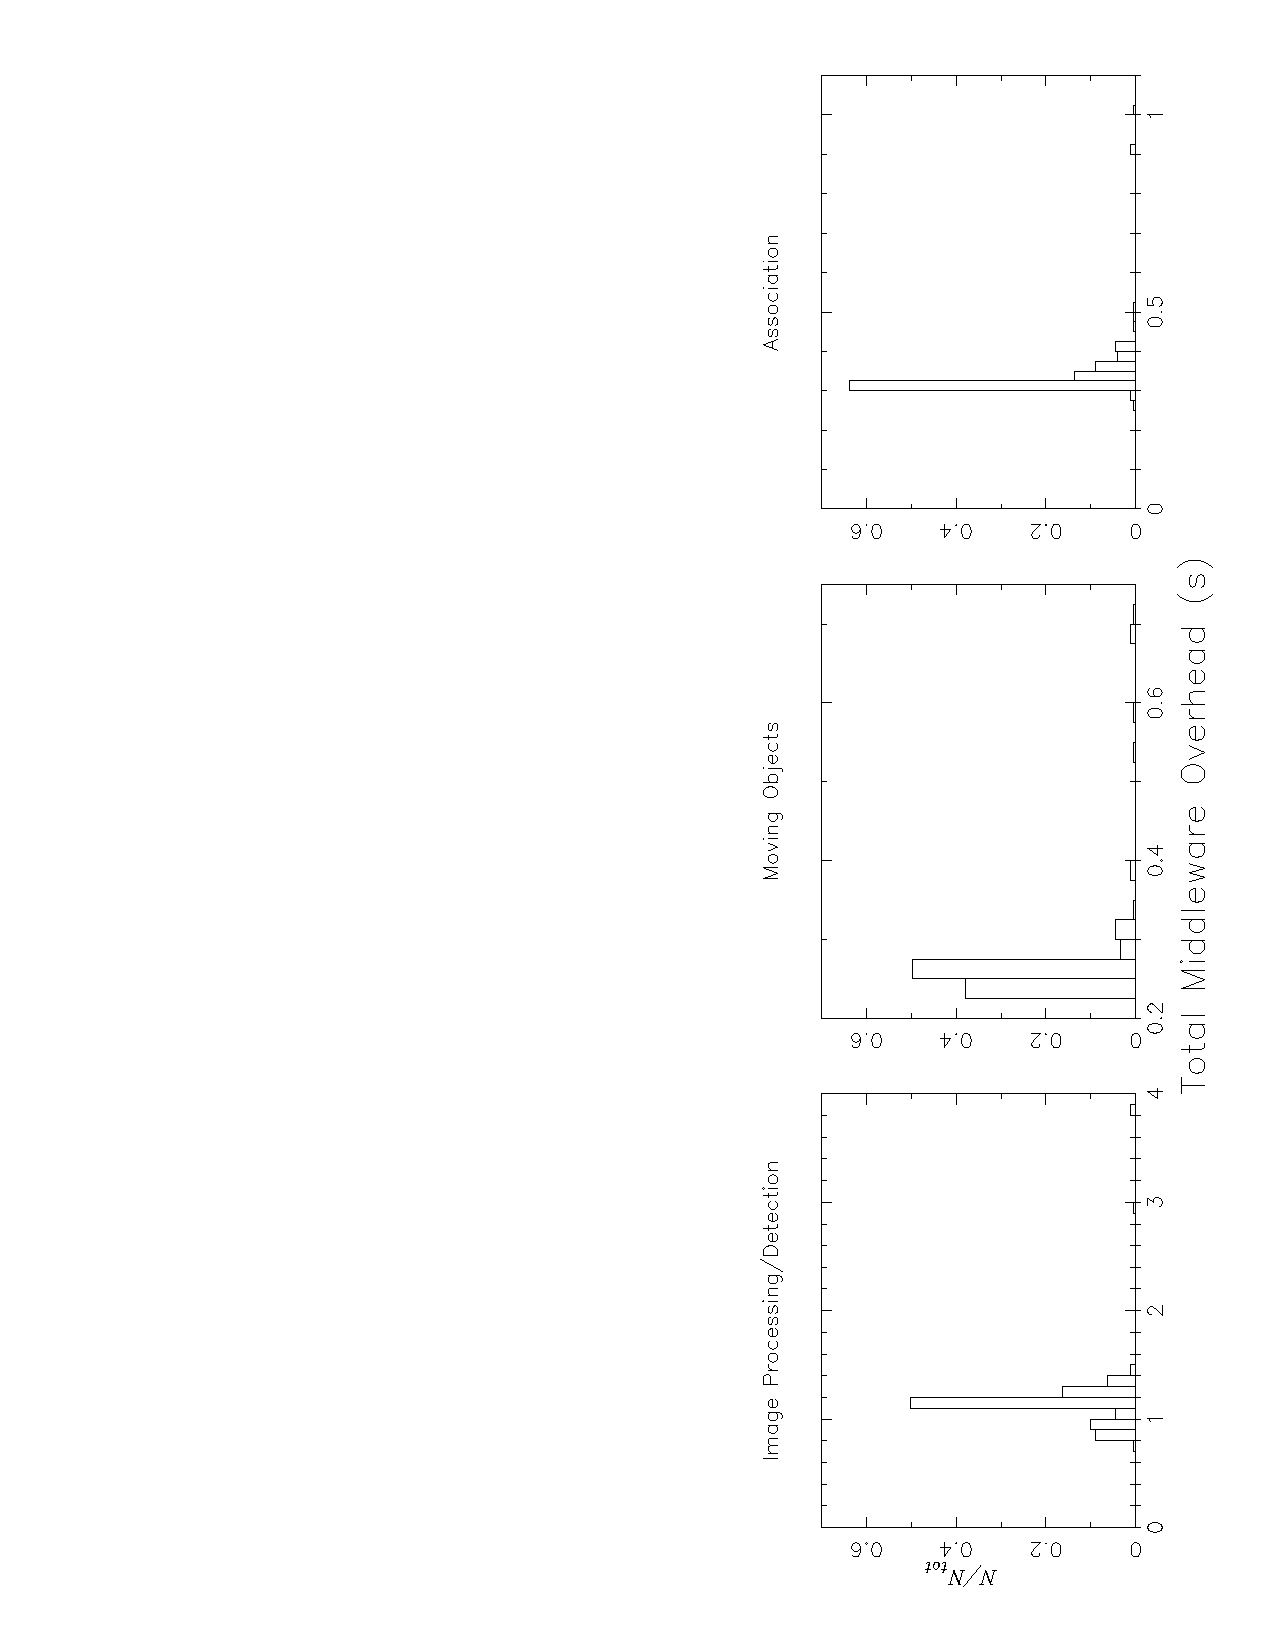
\includegraphics[width=0.8\textwidth,angle=-90,scale=0.375,viewport=364 29 583 757,clip]{figures/LoopOverhead.pdf}
\caption{Histogram of the overhead penalties --- that is, the time not
  spent in application code while processing one visit --- imposed by the pipeline
  framework.  The $y$-axis measures the fraction of the 177 visits in
  each time bin.\label{f6-7}} 

\vspace{0.5\baselineskip}

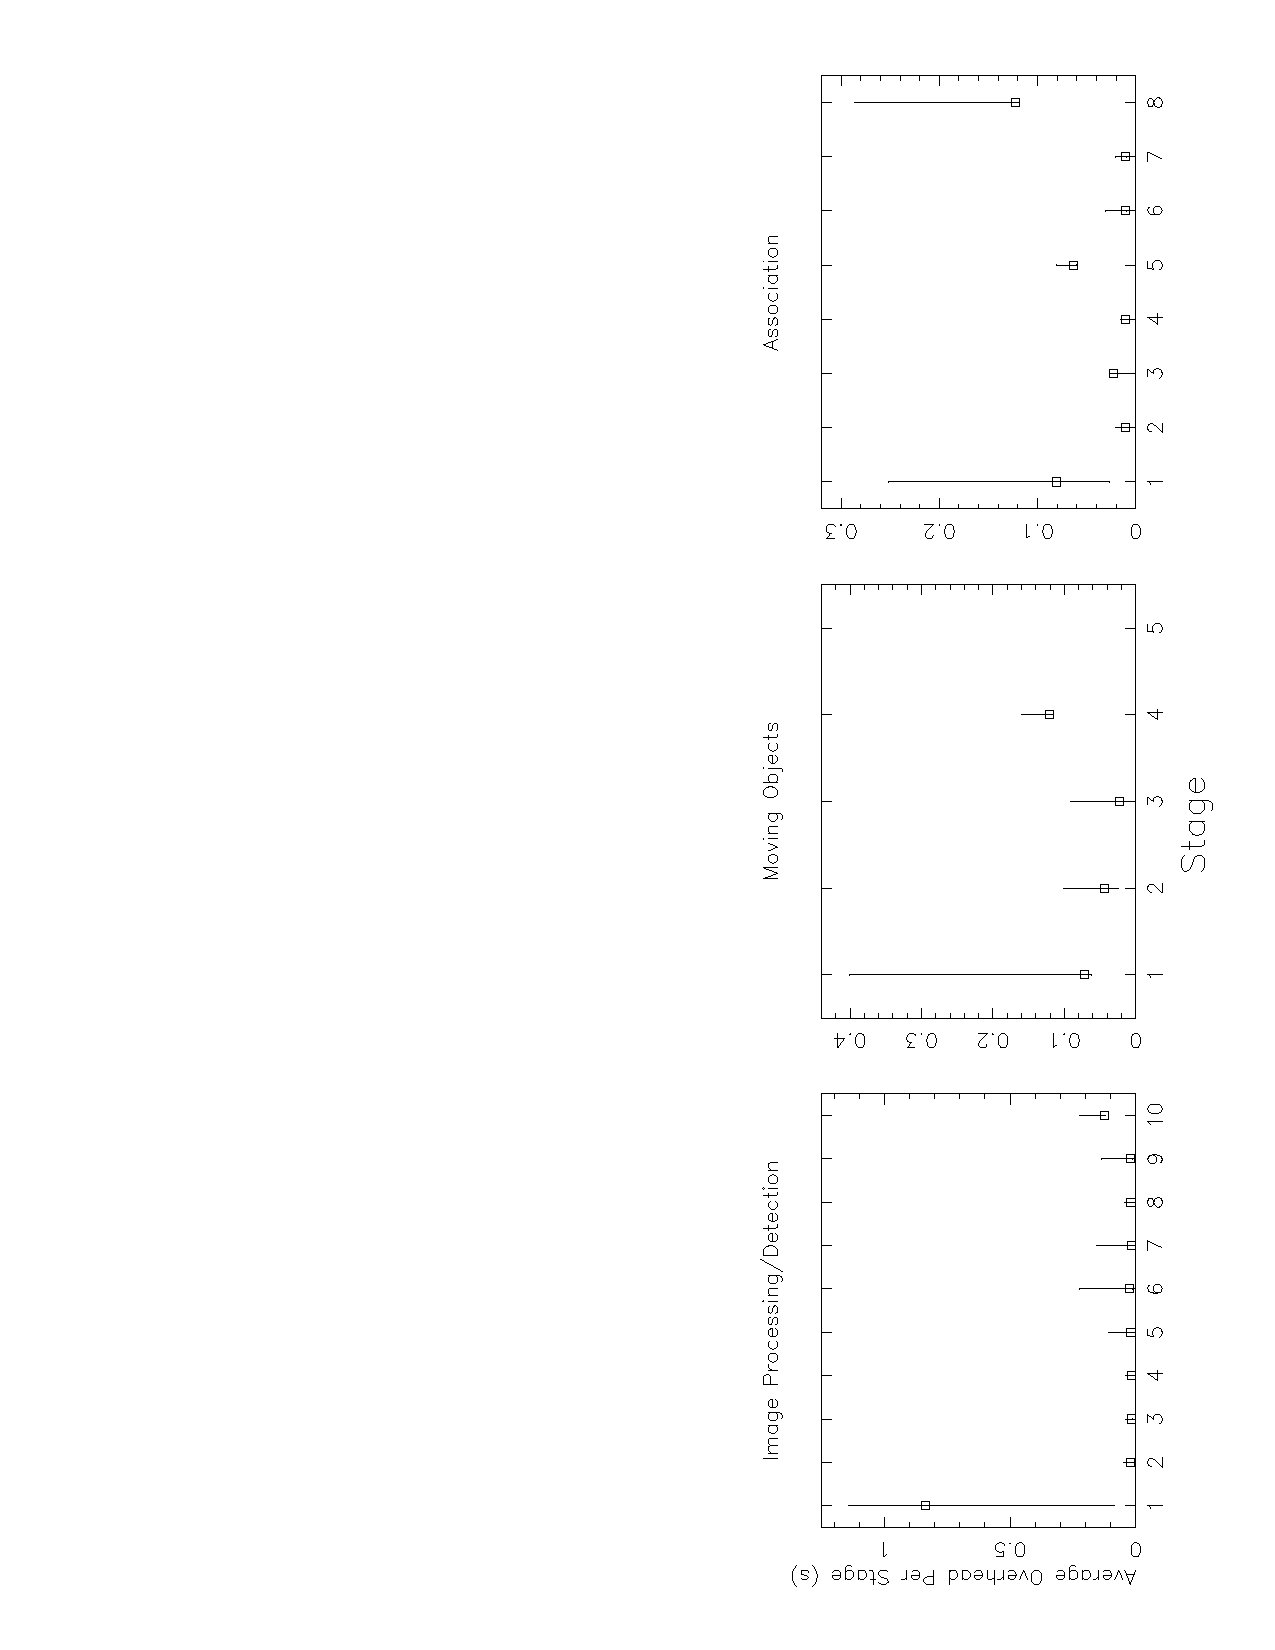
\includegraphics[width=0.8\textwidth,angle=-90,scale=0.375,viewport=364 29 583 757,clip]{figures/OverheadVsStage.pdf}
\caption{The average overhead times (represented by squares) as a
  function of stage for each pipeline.  The vertical lines through
  the squares extend to the minimum and maximum times. \label{f6-8}} 
\end{center}
\end{figure}

\begin{deluxetable}{lrr}
\tablecaption{Average overhead time per visit for each pipeline.\label{t6-4}}
\tablewidth{0pt}
\tablehead{
\colhead{Pipeline} & \colhead{avg. time (s)} & \colhead{$3\sigma$ (s)}
}
\startdata
Image Processing/Detection (IPD) &  1.17 & 1.03 \\
Moving Objects (MOPS)            &  0.27 & 0.20 \\
Association                      &  0.34 & 0.26 \\
\enddata
\\[-1.5\baselineskip]
\tablecomments{$N_{visits}=177$}
\end{deluxetable}

Because we can fairly accurately measure the time spent running actual
application code (covered in the \code{pre-process()}, \code{process()} and
\code{post-process()} steps), we can also measure the extra time that
the pipeline framework adds managing the pipeline; we refer to this as
the pipeline framework's \textit{overhead}.  Overhead is calculated on a
per visit basis, taking the total processing time for the visit (as
illustrated in \Fig{f6-4}) and subtracting the total time in
application code as well as the time spent waiting for an event to
arrive.  The averages of these overheads are summarized in
Table~\ref{t6-4} and illustrated in \Fig{f6-7}.  These results
show that the overhead is quite low (compared to the total processing
time).  \Fig{f6-7} shows that the overhead times are fairly
consistent.  \Fig{f6-8} shows how the overhead varies on
average as a function of the stage.  The overhead is larger on average
for the stages that receive events (stage 1 for all three pipelines
and stage 5 for the Association pipeline) and for the last stage after
which the clipboard must be cleaned up and restored.

\section{Conclusions}

% Tie in DC2 results to goals presented in Intro.
% Desired functionality in place
% Speed too slow, but isolated to convolution code; cause understood
% Science quality needs work - OK for DC2

We now refer back to the goals for DC2 presented in \Sec{Goals}, and
assess how they have been met.  To facilitate the discussion, it is
convenient to group the goals:

\begin{itemize}
\item Construction and demonstration of application framework and
  astronomical algorithms in the context of the LSST nightly processing pipeline.
\begin{itemize}
\item Demonstrate the use of astronomical algorithms for nightly
  processing in an LSST processing framework. 
\item Further develop and demonstrate common application framework
  functionality.
\item Establish an LSST simulated object/source database for testing
  by the broader collaboration.
\item Demonstrate integration of MOPS into LSST framework. 
\end{itemize}
\item Construct and demonstrate a middleware framework that
  supports the application framework.
\begin{itemize}
\item Update middleware implementation to enable the hosting and
  execution of application classes.
\item Demonstrate a database partitioning scheme.
\end{itemize}
\item Establish software development process that will persist through construction.
\begin{itemize}
\item Pilot the software development and testing process for future data
  challenges and the LSST construction phase.
\item Establish reusable code baseline for future data challenges and
  the LSST construction phase.
\end{itemize}
\end{itemize}

The goals for the application framework and for the algorithms implemented
using it have been nearly completely achieved, and this is clearly one of
the major results of DC2.  The prototype nightly processing pipelines
include the required algorithms, and have worked reliably as measured
by the fraction of input images that are successfully processed
through the pipeline. The one goal we have not achieved is establishing
a realistic object/source database for use by the broader collaboration.
While we have successfully implemented the database to the schema as
designed, and populated it with properly structured and linked data,
the data quality is not yet sufficient to be useful to the broader
collaboration.  The reasons for this are well understood, as discussed
in \Sec{ScienceDataQuality}, and much of the application code required
to achieve the goal has already been written and tested.

The innovation of the newly implemented pipeline harness is in the way
it effectively balances the use of Python and C++.  Application
Stages --- the container for the scientific algorithms --- can be written
with ease in Python.  These stage implemenations themselves can be
thin wrappers around our C++ classes.  Similarly, the pipeline harness
itself is a wrapper around a C++ implementation where the MPI control
calls are executed.  Our timing results show that the overhead added to
the total processing time by the pipeline harness is very small
compared to application processing time.  In particular, the overhead
scales linearly with the number of stages ($< 0.1$ seconds per stage) in
the absence of event processing.  Sending and receiving events adds
additional but still small overhead.  

Our pipeline harness does have a disadvantage that becomes apparent
when run on a heterogeneous cluster as we did.  Because of the way we
synchronize our processing, the overall speed of the pipeline is
limited by the performance of the slowest node.  This is important to
consider for the production system.  When we scale up to hundreds or
even thousands of cores and run nearly 24 hours a day, one or two
defective nodes could easily bring down the performance of the entire
cluster.  In future data challenges, we will look at strategies for
not only minimizing this effect, but also detecting when defective
nodes are having a major impact on performance.  

We have been quite successful in building up an effective software
development environment that not only builds the software via a few
simple commands but also manages all of the dependencies.  The ability
to have multiple versions of a package simultaneously, as provided by
the EUPS system, has been a very powerful feature, particularly during
the integration phase when many changes were coming in rapidly.  

Our package distribution system has also been an important mechanism
for our distributed team to keep up with the latest changes.  However,
the distribution system has suffered from two serious problems.  The first
has been in ensuring smooth installation of third party packages
across all of our development platforms.  While the differences
between the Mac and Linux platforms has been most challenging
(particularly for certain ``problem'' packages like Boost, CORAL, and
SEAL), supporting different distributions of Linux (particularly
64-bit Linux) has not been without problems.  Cross-platform support
issues for third-party packages have been the most common problem that
has prevented developers from getting the software stack installed on
their local environment.  The second problem stems from the amount of
time it takes to install a full software stack (as we build everything
from source).  This is not only a barrier to new developers but to
those of us who maintain the build and distribution system as it makes
debugging platform-dependent problems a slow process.  We hope our
future experiments with virtual machines will alleviate the barrier
for new developers.  

One observation that we have drawn from these problems is that
when the build environment runs well, the developer hardly notices it.
When it doesn't work, it can quickly disable a developer's progress.

\subsection{Required software developments for DC3}

As we prepare to transition from the completion of DC2 to the
development of DC3, it is appropriate to assess what improvements will
be required in the existing LSST software.  First, we emphasize that
our experience with the DC2 framework, and with the software
development system with which it was designed, built, and documented,
has been very positive.  We will use it as the foundation for DC3.

As we fully expected, however, we will need to extend it in various ways. The
preceding sections of this report have identified a number of detailed
improvements to the existing framework classes that we expect to need
for DC3.  We will not recap those here, rather taking a somewhat
higher level view.  The main required developments that we have
identified are:

\begin{itemize}

\item We need to define the role of the middleware orchestration layer in
   catching exceptions and possibly mediating adaptive behavior of the
   pipeline stages in recovering from problems such as algorithmic
   failures.

\item Need to define API and mechanism for inter-slice communication (not
   present or required for DC2).  We
   have at least three usecases that require some form of inter-slice
   communication: cross-talk correction; the association pipeline (which
   is currently using shared memory outside of the pipeline framework
   for this), and handling Footprints that cross amplifier boundaries

\item Related to inter-slice communication, the LSST focalplane, with
   its roughly 3000 amplifiers, 200 ccds, and 21 rafts, has lots of
   boundaries. We need to carefully assess where processing needs to take account of
   what's on the other side of a boundary.

\item We need to address the performance issues with accessing pixels
   under vw.  This is the source of our only significant performance problem.

\item We need to further develop the image subtraction software to
improve the data quality of the subtracted images.

\end{itemize}

\subsection{Scaling to LSST}

Finally, we need to assess where we stand in relation to the final
performance requirements for LSST.  The input images we have used for
DC2 have 340 Megapixels, just over 10\% the size of the LSST
focalplane.  They also have very similar pixel scale and somewhat
greater exposure depth as a single LSST exposure.  Although the
hardware available for DC2 prevented us from processing full images in
parallel, the DC2 software is designed to do so without modification.
We expect to make such runs shortly after completion of this report.
We are thus very close to processing a data stream that is 10\% that
of LSST.  This is in line with the expectations for DC2 set in the
MREFC proposal.

We do have a significant shortfall in the per-node performance on the
nightly processing pipeline, achieving about 20\% of what is required
to meet the 60 sec alert processing latency.  As discussed above, we
believe that we have isolated the performance problem to a small
section of code that utilizes the vw library (see \Sec{fwTiming}) to access image
pixels. Our strategy for verifying that we are on track to achieve the full LSST
performance level is to:

\begin{itemize}
\item Complete the full focalplane DC2 runs, utilizing 288 nodes for
  the IPD pipeline.  This will verify that the middleware framework is
  not limiting performance.
\item Work with the vw group at NASA Ames to resolve the pixel access
  performance issues that are limiting image subraction speed.
\item In the event that vw continues to be a performance issue, we
  will replace it.  The application APIs would not be significantly
  impacted by such a change, so changes to the existing software stack
  would be very localized.
\item As a risk reduction strategy, we will continue our ongoing
  effort to track and evaluate the performance of GPU and related
  architectures for image processing tasks.  Based on present
  application experience, these offer at least a factor of 4
  improvement in per-node performance, which gives ample headroom to
  meet full LSST performance.
\item We need to address load balancing issues inherent to our
  pipeline harness to ensure that a few defective nodes in a cluster
  do not drag down the performance of a massively parallel pipeline.  
\end{itemize}

We will have results from the first three steps in this plan by May, 2008.

